\documentclass[a4paper,11pt]{article}
\usepackage[T1]{fontenc}
\usepackage[polish,english]{babel}
\usepackage[utf8]{inputenc}
\usepackage{lmodern}
\usepackage{graphicx}
\usepackage[font=small,labelfont=bf]{caption}
\usepackage{pdflscape}

\title{Sauron}
\author{Mateusz Forc, \\ Grzegorz Staniszewski, \\ Wiktor Franus, \\ Przemysław Kopański}

\begin{document}

\selectlanguage{polish}

\maketitle
\tableofcontents

\newpage
\section{Treść zadania}
W pierścieniu połączone są serwer i N czujników.
Serwer jest stale aktywny. Czujniki periodycznie budzą się i wykonują pomiar.
Każdy czujnik próbuje odebrać komunikat z pomiarami od jednego sąsiada i wysłać drugiemu sąsiadowi.
Czujniki oszczędzają energię, zatem należy minimalizować czas ich pracy i wolumin
transmitowanych danych.
Sieć ma tolerować pojedyncze uszkodzenie węzła lub połączenia.
Należy zaprojektować i wykonać system komunikacji dla tej sieci.
Przeanalizować wybór protokołu IPv4 i IPv6.
Ponadto należy zaprojektować moduł do Wireshark umożliwiający wyświetlanie i analizę
zdefiniowanych komunikatów.

\section{Założenia funkcjonalne}

\begin{enumerate}
  \item Serwer
  \begin{enumerate}
    \item inicjalizuje sieć czujników
    \item ustala tryb pomiaru wspólny dla wszystkich czujników
    \item uruchamia pomiar
    \item przechowuje informacje o czujnikach oraz wykonywanych pomiarach
    \item rozpoznaje miejsca awarii sieci i wypisuje komunikaty
    \item w przypadku awarii dowolnego czujnika przystosowuje sieć do możliwie poprawnego funkcjonowania
  \end{enumerate}
  \item Czujnik
  \begin{enumerate}
    \item periodycznie budzi się, wykonuje pomiar i przesyła go do serwera
    \item przekazuje odbierane wiadomości w stronę docelowego urządzenia
  \end{enumerate}
  \item Aplikacja wspiera IPv4 i IPv6.
  \item Konfiguracja sieci pobierana jest z pliku.
\end{enumerate}

\section{Założenia niefunkcjonalne}

\begin{enumerate}
  \item Serwer jest stale aktywny.
  \item Sieć ma tolerować uszkodzenia węzłów lub połączeń.
  \item Minimalizacja czasu pracy czujników i ilości transmitowanych danych.
\end{enumerate}

\section{Przypadki użycia}\label{PU}

\subsection{Włączenie systemu}
Aktorzy: użytkownik\\
Scenariusz główny:
\begin{enumerate}
   \item Użytkownik wprowadza do pliku konfiguracyjnego adresy czujników i tryb pomiaru
   \item Użytkownik uruchamia aplikację (serwer)
   \item Serwer inicjalizuje czujniki
   \item Serwer wypisuje komunikat o sukcesie
   \item Serwer rozpoczyna wykonywanie pomiarów przez czujniki
   \item Serwer wypisuje na ekran pomiary otrzymane z czujników
\end{enumerate}
Scenariusz alternatywny 1: (Jeden czujnik nie działa na etapie inicjalizacji)
\begin{enumerate}
   \item [1-3.] Jak w scenariuszu głównym
   \item [4.] Serwer wypisuje ostrzeżenie z informacją o niedziałającym czujniku
   \item [5-6.] Jak w scenariuszu głównym
\end{enumerate}
Scenariusz alternatywny 2: (Jeden czujnik przestaje działać po etapie inicjalizacji)
\begin{enumerate}
   \item [1-5.] Jak w scenariuszu głównym
   \setcounter{enumi}{5}
   \item Serwer wypisuje ostrzeżenie z informacją o niedziałającym czujniku
   \item Serwer wypisuje na ekran pomiary otrzymane z czujników
\end{enumerate}
Scenariusz alternatywny 3: (Więcej niż jeden czujnik przestaje działać po etapie inicjalizacji)
\begin{enumerate}
   \item [1-5.] jak w scenariuszu głównym
   \setcounter{enumi}{5}
   \item Serwer wypisuje komunikat o awarii systemu
   \item Serwer usypia działające czujniki
   \item Serwer kończy działanie jak w PU \ref{turnoff}
\end{enumerate}

\subsection{Wyłączenie systemu}\label{turnoff}
Scenariusz główny:
\begin{enumerate}
   \item Serwer usypia działające czujniki
   \item Serwer kończy działanie
\end{enumerate}

\subsection{Wyłączenie systemu przez użytkownika}
Scenariusz główny:
\begin{enumerate}
   \item Użytkownik zleca serwerowi zakończenie pracy
   \item Serwer kończy działanie jak w PU \ref{turnoff}
\end{enumerate}

\section{Wybranie środowisko sprzętowo-programowe i narzędziowe}

\begin{enumerate}
  \item System operacyjny: GNU Linux (dystrybucje: ArchLinux, Ubuntu)
  \item Języki programowanie: C, C++ (aplikacja), Lua (wtyczka do Wireshark)
  \item Kompilatory: GNU C++ Compiler, Clang
  \item Biblioteki: API gniazd BSD, Boost, YAML-CPP
  \item Narzędzia pomocnicze: Git, Gerrit, Github, gdb, CMake, Wireshark, Jenkins, Docker
\end{enumerate}

\newpage
\section{Architektura rozwiązania}
Architektura rozwiązania jest hybrydą architektur pierścieniowej oraz klient-serwer.
W sieci pierścieniowej połączone są ze sobą czujniki - dokonujące pomiaru, wraz z serwerem głównym -
zbierającym wyniki oraz zestawiającym całą sieć do poprawnej transmisji. Dodatkowo,
czujniki pełnią rolę serwera pośredniczącego; ze względu na budowę sieci muszą one
odbierać i przekazywać wyniki pomiarów innych czujników oraz informacje organizacyjne sieci.

\begin{center}
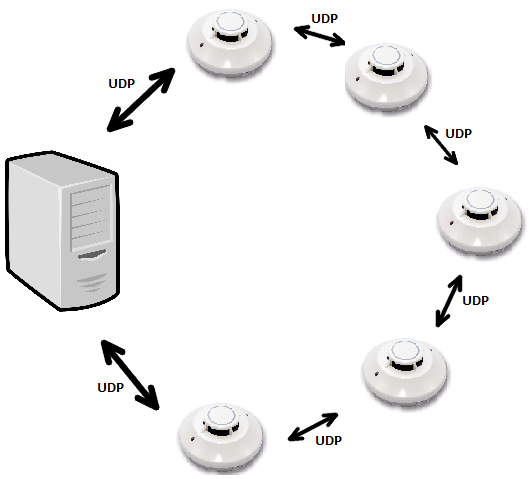
\includegraphics[scale=0.5]{architektura}
\end{center}

\subsection{Inicjalizacja}
Serwer trzyma listę adresów IP należących do pierścienia.
Wyznacza nastepnie podziałkę w ich połowie - od tej pory komunikacja będzie odbywać się tylko w dwóch
połowach pierścienia niezależnie (oszczędzamy wolumin danych i ułatwiamy zarządzanie nimi w normalnym trybie pracy).
Do wyznaczonych połówek wysyłane są adresy określające połowy pierścienia wraz z kierunkiem
przesyłania pomiarów. Serwer oczekuje na informację zwrotną z obu połówek świadczącą o braku
błędów podczas inicjalizacji. Każdy czujnik po wysłaniu wiadomości oczekuje na odpowiedź,
co umożliwia wykrycie awarii sieci.

\newpage
Czujnik pracuje w dwóch trybach naprzemiennie:
\begin{itemize}
\item w trybie aktywnym (okienko czasowe), 
	  w którym dokonuje pomiaru i przekazuje w kierunku serwera pomiary dokonane      przez inne wezły sieci.
\item w trybie nieaktywnym, w którym nasłuchuje tylko na wybrane komunikaty
\end{itemize}

\subsubsection{AWARIA 1: węzeł nie odpowiada podczas inicjalizacji}
Węzeł, który nie otrzymał odpowiedzi zwrotnej od sąsiada podczas inicjalizacji,
zwraca w przeciwną stronę informację o błędzie zawierającą adres IP węzła, który nie odpowiedział.
Informacja z błędem trafia ostatecznie do serwera.
Serwer rozpoczyna inicjalizację czujników od początku,
dostosowując listy adresów czujników w obu połówkach pierścienia,
w sposób umożliwiający poprawną komunikację z jednym niedziałającym czujnikiem.
%dodac rysunek jak zostaly wezly podzielone,
%ktory to jest wezel graniczny, i w ktorym kierunku nastepuje przesylanie pomiarow

\subsection{Tryb pomiaru}
Pomiary startują po otrzymaniu od serwera wiadomosci RUN.
Węzły wysyłają wynik pomiaru w stronę serwera; każdy z nich, jeżeli otrzyma od sąsiada pomiar, przekazuje go dalej w odpowiednią stronę.
Po każdej wysłanej wiadomości węzeł oczekuje na jej potwierdzenie od sąsiedniego węzła, brak potwierdzenia oznacza awarię węzła.

\subsubsection{AWARIA 2: węzeł nie odpowiada podczas zbierania wyników pomiarów}
Węzeł, który nie otrzymał potwierdzenia od adresata wiadomości zawierającej pomiaru,
wysyła w przeciwnym kierunku tą samą wiadomość dodając do niej informację o adresie wadliwego węzła.
Czujnik znajdujący się po drugiej stronie wadliwego węzła,
nie otrzymawszy w dopuszczalnym czasie od poprzednika żadnej wiadomości,
przesyła do kolejnego węzła swój pomiar dołączając do wiadomości adres wadliwego węzła.
Serwer z dwóch stron otrzymuje informację o pomiarach i wadliwym czujniku.
Jeśli adresy otrzymane z dwóch stron są różne to zaszła awaria więcej niż jednego czujnika.
Serwer przystępuje wtedy do wyłączania czujników. Jeśli serwer otrzymał od obu sąsiadów
ten sam adres wadliwego czujnika, oznacza to, że tylko jeden węzeł doznał awarii.
W tym przypadku serwer dokonuje ponownej inicjalizacji sieci dostosowując odpowiednio listę
adresów IP w obu połówkach pierścienia.

%goodbye + errors

\section{Sposób testowania}
\begin{itemize}
  \item Testy jednostkowe dla wszystkich modułów napisane w Boost Test Unit
  \item Testy integracyjne
  \item Możliwość uruchomienia wszystkich rodzajów testów za pomocą jednego polecenia
\end{itemize}

\section{Sposób demonstracji rezultatów}
Działanie systemu zostanie zaprezentowane przy pomocy narzędzia Docker,
przy pomomcy którego zostanie stworzona wirtualna sieć pierścieniowa, w której dokona się poprawna innicjalizacja, a następnie rozpocznie się wykonywanie pomiarów.

\section{Opis struktury implementacyjnej systemu}
Serwer wewnętrznie składa się z 3 obiektów - jeden główny zarządca oraz 2 podpierścienie. Główny wątek pobiera wiadomości z sieci i przekazuje je do odpowiedniego wątku półpierścienia. Synchronizuje ze sobą pracę obu podrzędnych wątków. Wątek półpierścienia zestawia połączenie i ponosi odpowiedzialność za komunikację w swoim obrębie.

\begin{landscape}
  \pagestyle{empty}
\begin{center}
    \centerline{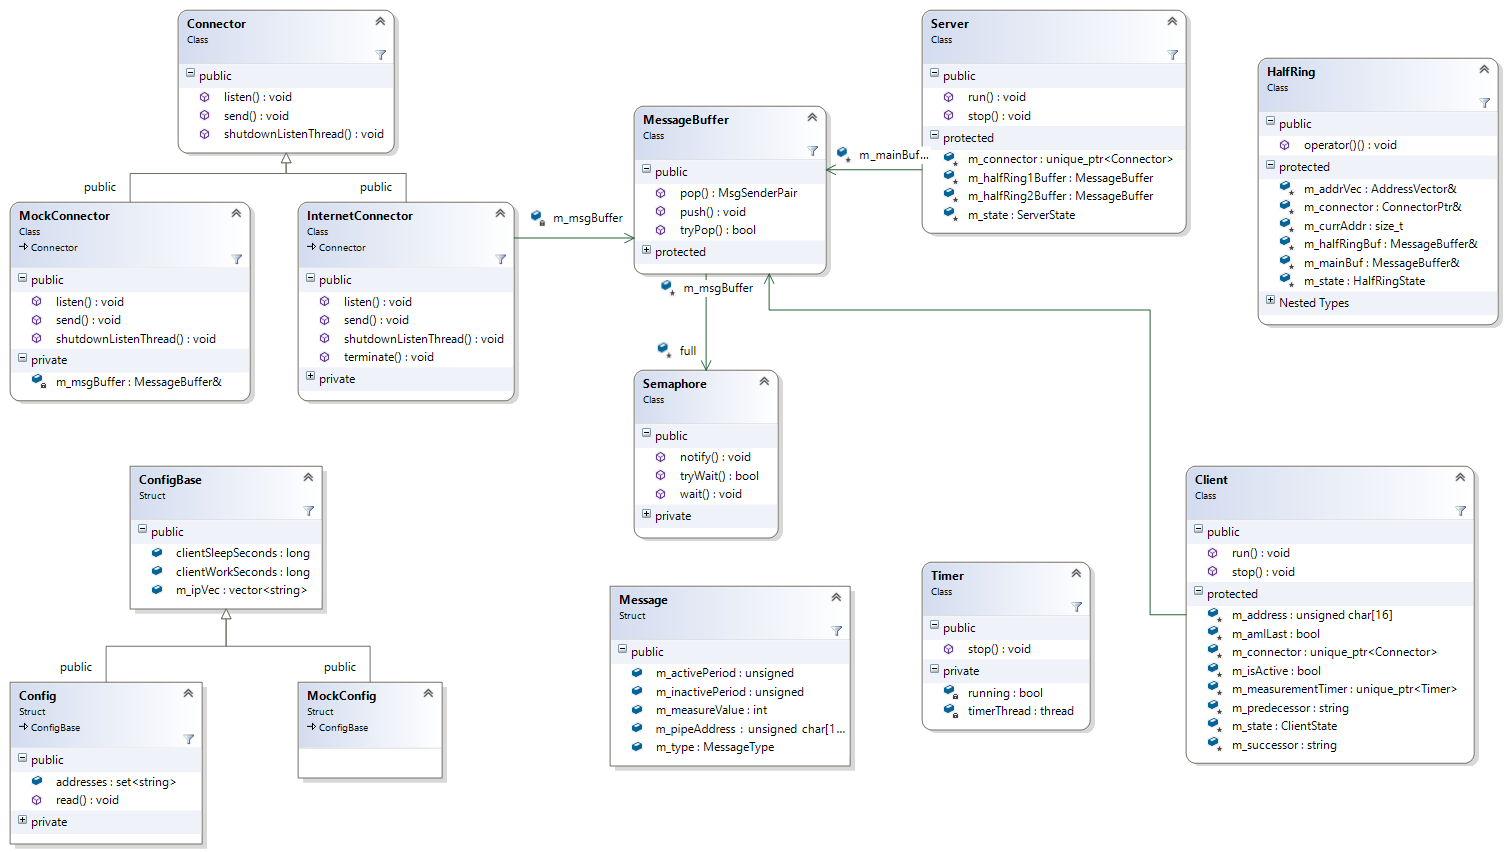
\includegraphics[width=1.4\textwidth]{class_diagram}}
    \captionof{figure}{Diagram klas wykorzystywanych w aplikacji}
\end{center}
\end{landscape}
\newpage


\section{Definicja komunikatów}
%ich strukturę (tj. typy parametrów) i sposób ich kodowania,
%określenie kto jakie komunikaty odbiera i wysyła.
Komunikacja między węzłami sieci odbywa się przy użyciu zdefiniowanej przez nas
struktury Message:

\begin{verbatim}
struct Message {
    // wyliczeniowy typ wiadomości
    MessageType m_type;

    // adres IP wykorzystywany przy inicjalizacji i podczas wykonywania pomiarów
    unsigned char m_pipeAddress[16];

    // wynik pomiaru
    int m_measureValue;

    // czas pracy czujnika (w sek.)
    unsigned m_activePeriod;

    // czas "spania" czujnika (w sek.)
    unsigned m_inactivePeriod;
};
\end{verbatim}

Pole m\_type w strukturze Message może przyjmować jedną z wartości typu wyliczeniowego
MessageType:

\begin{itemize}
\item \textbf{Init} - wysyłane przez serwer na etapie inicjalizacji w celu dołączenia do sieci kolejnego węzła. W polu m\_pipeAddress znajduje się adres IP dodawanego węzła. Czujniki otrzymując wiadomość tego typu po raz pierwszy, dołączają się do sieci (czujnik zapamiętuje adres poprzednika) i wysyłają w stronę serwera wiadomość typu InitOk. Kolejne odebranie wiadomości tego typu skutkuje zapamiętaniem adresu następnego węzła w pierścieniu i przekazaniem mu tej wiadomości.
\item \textbf{InitOk} - wysyłane przez świeżo dołączonego do sieci klienta w stronę serwera
\item \textbf{InitLast} - wysyłane dwukrotnie przez serwer do ostatniego klienta w półpierścieniu. Za pierwszym razem pole m\_pipeAdress zawiera adres ostatniego węzła należącego do półpierścienia. Za drugim - adres ostatniego węzła z drugiej połowy pierścienia. Niezainicjalizowany do tej pory klient (ostatni) otrzymawszy kolejno dwie takie wiadości zapamiętuje swój adres, awaryjny adres sąsiada z drugiej połowy pierścienia oraz informację o swoim krańcowym położeniu w półpierścieniu.
\item \textbf{Run} - wysyłane przez serwer do pierwszych klientów w półpierścieniach. Klient przekazuje tą wiadomość następnikowi, sam rozpoczynając pierwszy pomiar.
\item \textbf{Measurement} - wysyłane przez klienta w stronę serwera. W polu m\_pipeAddress umieszczony jest adres czujnika, który wykonał pomiar. Wynik pomiaru znajduje się w  polu m\_measureValue.
\item \textbf{Finish} - wysyłane przez serwer do klienta podczas wyłączania systemu. Klient przekazuje wiadomość do następnika i kończy działanie. Używane również wewnątrz modułu serwera do informowania wątków obługujących półpierścienie o zakończeniu działania aplikacji.
\item \textbf{Ack} - wysyłane przez węzeł sieci (serwer lub klient) do nadawcy poprzednio odebranej przez węzeł wiadomości (potwierdzenie odebrania).
\item \textbf{Terminate} - pomocniczy typ używany wewnątrz modułów serwera i klienta (nie przesyłany przez sieć).
\item \textbf{OneHalfInitFinish} - pomocniczy typ używany wewnątrz modułu serwera. Wiadomość tego typu umieszczana jest w buforze wątku głownego przez wątek obłsugujący półpierścień po pomyślnej inicjalizacji obsługiwanych czujników.
\end{itemize}

\section{Opis zachowania podmiotów komunikacji}
%% TODO: opisać co się dzieje wewnątrz serwera - współpraca Server i HalfRing

\subsection{Diagramy stanów}
\begin{center}
	\centerline{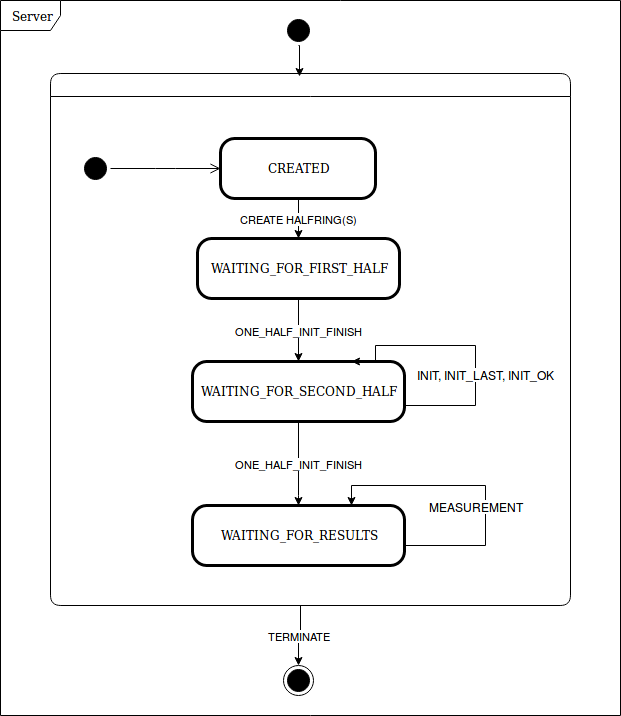
\includegraphics[width=1.0\textwidth]{server_states}}
	\captionof{figure}{Diagram stanów głównego wątku serwera.}
\end{center}
\begin{center}
	\centerline{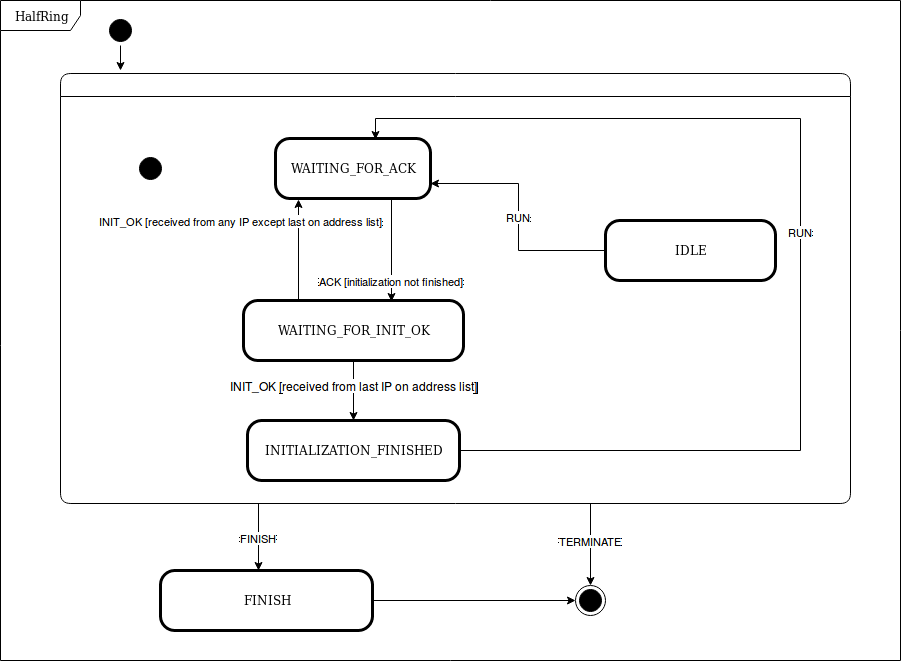
\includegraphics[width=1.2\textwidth]{halfring_states}}
	\captionof{figure}{Diagram stanów wątku obsługującego połowę pierścienia czujników.}
\end{center}
\begin{center}
	\centerline{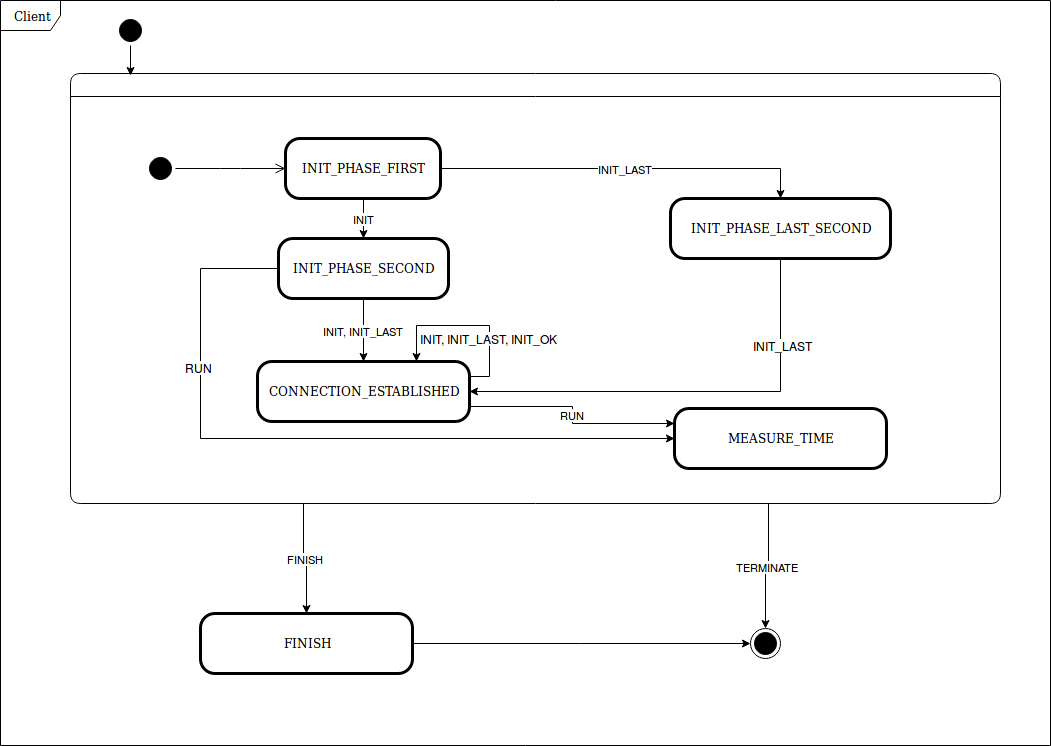
\includegraphics[width=1.2\textwidth]{client_states}}
	\captionof{figure}{Diagram stanów klienta.}
\end{center}

\subsection{Opis zegarów klienta}
Z każdym z czujników związany jest zegar, który wyzwala dokonanie pomiaru. Wykonany pomiar jest natychmiast wysyłany w stronę serwera. Przez pozostały czas trwania 'okienka czasowego' czujnik nasłuchuje na pomiary od sąsiadów i przekazuje je dalej. Po upłynięciu czasu pracy czujnik jest usypiany na okres trwania czasu nieaktywności. W tym czasie wszystkie odebrane komunikaty są ignorowane. Kolejne wyzwolenie zegara rozpoczyna nowy pomiar. Czas między kolejnymi pomiarami równy jest zatem sumie czasu pracy i czasu 'spania' czujników.

\subsection{Scenariusze komunikacji}
%wyrażone np. w MSC lub w innych diagramach komunikatów.
%\begin{figure}
\begin{center}
	\centerline{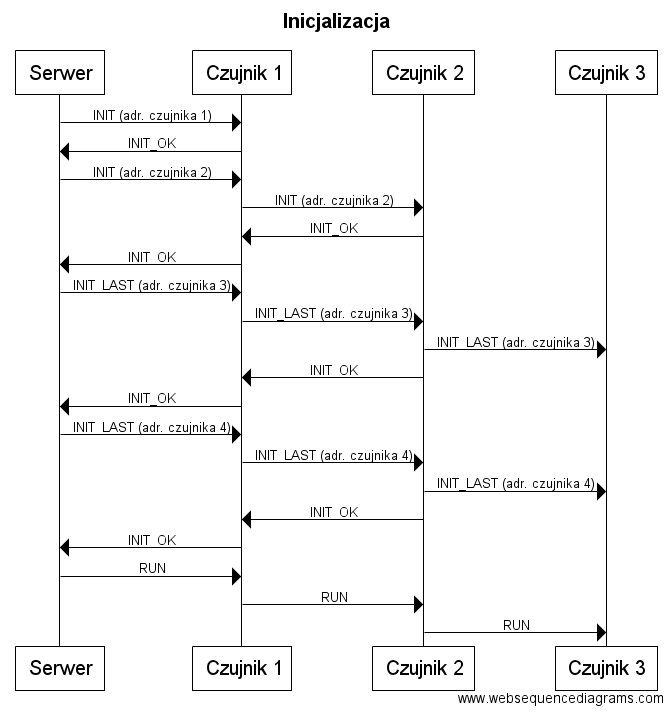
\includegraphics[width=1.3\textwidth]{init_seq}}
	\captionof{figure}{Sekwencja komunikatów podczas inicjalizacji sieci. Czujniki 1,2 i 3 należą do tego samego półpierścienia. Czujnik 4 (nie umieszczony na rysunku) jest ostatnim węzłem z drugiej połowy pierścienia.}
	\centerline{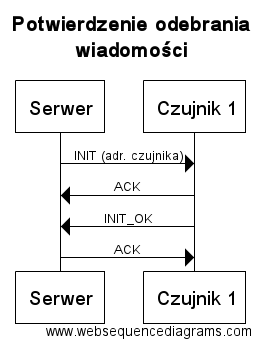
\includegraphics[width=0.4\textwidth]{ack_seq}}
    \captionof{figure}{Przykładowa sekwencja przedstawiająca potwierdzenie otrzymania wiadomości przez węzeł w sieci.}
    \centerline{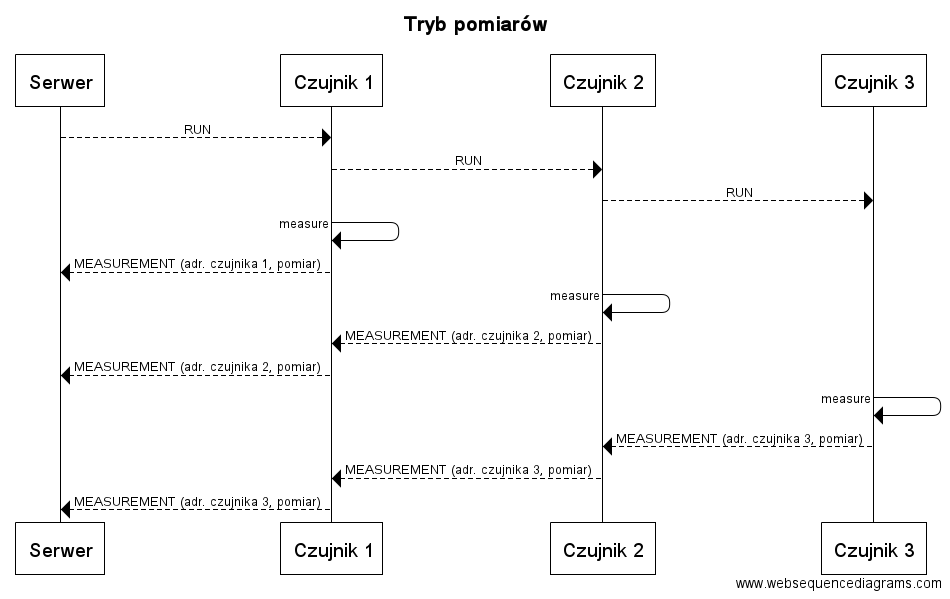
\includegraphics[width=1.4\textwidth]{measure_seq}}
    \captionof{figure}{Sekwencja komunikatów podczas rozpoczynania etapu pomiarów.}
    \centerline{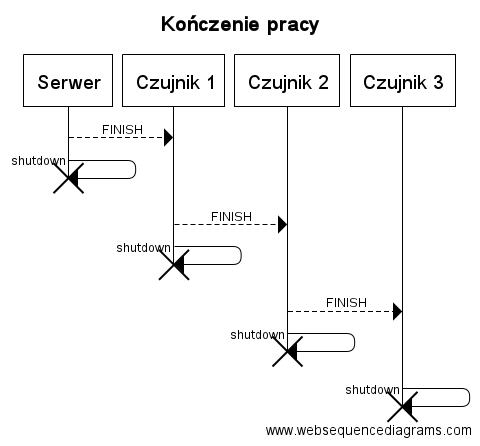
\includegraphics[width=1.0\textwidth]{finish_seq}}
    \captionof{figure}{Sekwencja komunikatów podczas kończenia pracy systemu.}
\end{center}

\section{Wnioski z wykonanego testowania}
Aplikacja z racji na wielowątkowość, wykorzystywanie protokołu sieciowego oraz ścisłe powiązanie serwera/klienta z konkretnym portem jest problematyczna w testowaniu. Integracja serwera oraz kilku instancji klienta bez wykorzystania izolowanych wirtualnych środowisk jest w zasadzie niemożliwa. \\
Testowanie jest procesem znacznie bardziej kosztownym czasowo niż implementacja, jednak jest to proces, w który warto inwestować czas i pieniądze gdyż zwiększa on jakość projektu oraz daje poczucie deweloperom, iż wprowadzane przez nich zmiany nie popsują działającego już kodu.

\section{Podział prac w zespole}
Prace nad projektem wykorzystują jedną z metod programowania zwinnego,
tj. pair programming - każde zadanie przydzielane jest parze.
Pary oceniają nawzajem stworzony przez siebie kod przy uzyciu narzędzia do rewizji kodu Gerrit.
Istnieją zadania, które wykonuje cały zespół lub sam lider. \\
Przydział zadań:
\begin{enumerate}
\item Sprint 1 - dokumentacja wstępna i repozytorium
\begin{itemize}
\item Stworzenie dokumentacji wstępnej - cały zespół
\item Utworzenie repozytorium na Github - Mateusz Forc (lider)
\item Integracja repozytorium z Gerrit - Mateusz Forc (lider)
\item Założenie kont dla programistów oraz prowadzącego - Mateusz Forc (lider)
\item Stworzenie instrukcji korzystania z Gerrit oraz ustalenie stylu kodowania
      - Mateusz Forc (lider)
\end{itemize}
\item Sprint 2 - implementacja podstawowych funkcjonalności
\begin{itemize}
\item Projekt komunikatów - cały zespół
\item Wtyczka do Wireshark - Przemysław Kopański
\item Wrapper API gniazd BSD - Mateusz Forc (lider), Wiktor Franus
\item Testy jednostkowe wrappera w zakresie podstawowym - Mateusz Forc (lider), Wiktor Franus
\item Projekt i implementacja modułu serwera wraz z podstawowymi funkcjonalnościami
      - Mateusz Forc (lider), Wiktor Franus
\item Projekt i implementacja modułu klienta (czujnika) wraz z podstawowymi funkcjonalnościami
      - Grzegorz Staniszewski, Przemysław Kopański
\item Testy jednostkowe modułów serwera w zakresie podstawowym - Mateusz Forc (lider), Wiktor Franus
\item Testy jednostkowe modułów klienta w zakresie podstawowym
      - Grzegorz Staniszewski, Przemysław Kopański
\item Podstawowe testy integracyjne aplikacji - Grzegorz Staniszewski, Przemysław Kopański
\item Zaprojektowanie i implementacja klasy bufora wiadomości - Przemysław Kopański
\item Budowanie aplikacji z użyciem narzędzia CMake - cały zespół
\item Poprawa stylu kodowania - Grzegorz Staniszewski
\item Zmiana struktury katalogów w projekcie - Mateusz Forc (lider), Wiktor Franus
\item Utworzenie i skonfigurowanie zadań w narzędziu Jenkins (ciągła integracja) - cały zespół
\end{itemize}
\item Sprint 3 - kompletna implementacja wraz ze wszystkimi testami
\begin{itemize}
\item Uzupełnienie testów jednostkowych wrappera - Mateusz Forc (lider), Wiktor Franus
\item Bezpieczne zamykanie aplikacji wraz z jej wszystkimi wątkami i zwalnianiem zasobów - cały zespół
\item Projekt i implementacja zegarów synchronizujących pracę czujników - Przemysław Kopański
\item Utworzenie i konfiguracja środowiska do testów akceptacyjnych - Przemysław Kopański
\item Implementacja pozostałych funkcjonalności modułu serwera - Mateusz Forc (lider), Wiktor Franus
\item Wczytywanie konfiguracji sieci z pliku - Grzegorz Staniszewski
\item Implementacja pozostałych funkcjonalności modułu klienta
      - Grzegorz Staniszewski, Przemysław Kopański
\item Pozostałe testy modułu serwera - Mateusz Forc (lider), Wiktor Franus
\item Pozostałe testy modułu klienta - Grzegorz Staniszewski, Przemysław Kopański
\item Uodpornienie programu na niepożądane parametry od użytkownika
      - Grzegorz Staniszewski
\item Aktualizacja zadań w sprincie 2 i 3 w ramach dokumentacji - Mateusz Forc (lider), Wiktor Franus
\item Aktualizacja dokumentacji przed oddaniem projektu - cały zespół
\item Poprawa nagłówków w plikach z kodem źródłowym  - Mateusz Forc (lider), Wiktor Franus
\item Aktualizacja zadań na GitHubie w oparciu o narzędzie Gerrit oraz dokumentację - Mateusz Forc (lider)

\end{itemize}
\end{enumerate}

\section{Harmonogram prac}
Sprint 2 - od 19.04 do 15.05 \\
Sprint 3 - od 15.05 do 31.05 \\

\section{Podsumowanie}
\subsection{Niezrealizowane założenia funkcjonalne}
Ze względu na napięte wymagania czasowe i jednoczesną chęć zrealizowania projektu wysokiej jakości, zdecydowaliśmy sie ograniczyć zakładaną funkcjonalność o następujące założenia: 
\begin{itemize}
    \item serwer rozpoznaje miejsca awarii sieci i wypisuje komunikaty,
    \item w przypadku awarii dowolnego czujnika serwer przystosowuje sieć do możliwie poprawnego funkcjonowania.
\end{itemize}
Zaimplementowane cechy systemu zapewniają poprawną pracę w przypadku braku awarii w sieci.

\subsection{Opis wyniesionych doświadczeń z realizacji projektu}
Praca z interfejsem gniazd BSD była uciążliwa, a popełnione błędy trudne do wykrycia podczas pisania. W przyszłych projektach wymagających użycia komunikacji sieciowej zdecydujemy się z pewnością na użycie gotowych, przetestowanych i bardziej abstrakcyjnych bibliotek \\
Realizacja projektu pozwoliła nam na poszerzenie znajomości języka C++ poprzez praktyczne stosowanie funkcji z najnowszych bibliotek standardowych. Korzystanie z narzędzi Gerrit i Git stało się dla niektórych członków zespołu nową umiejętnością, która z pewnością zostanie przez nich użyta w pracy zawodowej.\\
Ciekawym i równie owocnym doświadczeniem była praca w parach, która niosła ze sobą wiele pozytywnych efektów, m.in. przyjemniejszą pracę nad kodem, szybsze rozwiązywanie problemów, dzielenie się wiedzą z kolegami i pogłebianie stosunków międzyludzkich.

\subsection{Statystyki rozmiarów stworzonych plików}
Liczba linii w plikach źródłowych: ok. 1800 \\
Liczba linni w plikach z testami: ok. 1000 \\
Wtyczka do Wireshark: ok. 60

\subsection{Czas poświęcony na realizację projektu w godzinach}
Realizacja projektu, w skład której oprócz projektowania i implementacji wchodziły także
spotkania konsultacyjne i etapowe pochłonęła około 280 osobogodzin (średnio 70h na osobę).

\section{Adres projektu}
Repozytorium kodu dostępne jest w serwisie Github pod adresem:
\begin{center}https://github.com/formateu/sauron \end{center}
Dostęp do repozytorium jest ograniczony do kont posiadających uprawnienia do jego odczytu.
\end{document}
\grid
